\clearpage
\section{Sensors}
\subsection{Pressure Based}
Pressure based sensors work by simply measuring how much pressure there is in a point in space. They can be used to measure the vertical distance between two points in a planet with an atmosphere\cite{barometric1}\cite{barometric2}. By combining height information with the data gathered by other sensors, it is possible to create a crude three-dimensional map.

\subsection{Image Based}
Image based sensors are usually just cameras. The pictures the sensor takes, must be mathematically processed to yield any useful data. The two most common types of image sensors are stereoscopic and projected.

A projected image sensor is very simple, some known image is projected on the environment (a grid, for example), then a camera takes a picture. Since the projection is known, it is simple to detect the distance of an object on the image based on what the projection looks like. This method is limited to how fine the projected image is.

Stereoscopy is more complicated, but more reliable. Two photos of the same scene, but from different vantage points, are taken. Small sections of one of the images are taken, and overlayed onto the other image. By finding the place on the other image where the small section fits, the algorithm can determine the depth of each pixel in that subsection. This procedure is repeated until the whole image has been processed.

\subsection{Rangefinder}%NOTE: This section might be a little rambly
A rangefinder is a device that measures the distance between itself, and a point some distance away from it. Rangefinders work based on the principle that the speed of an object is defined to be distance travelled over time travelled, which means that distance travelled is the speed of an object times the amount of time it travelled. To put this in math terms: \{v=d/t\} or \{d=t*v\}.

Most rangefinders work on either sound or light. Both sound and light based rangefinders work by emitting a pulse in a specific direction, and counting how long it takes for the pulse to come back. Since the pulse has travelled back and forth, the distance is calculated as \(1/2*v*t\), where \(v\) is the speed of the pulse, and \(t\) is the time between the emission and the detection.

The pulse will travel from the rangefinder, straight to whatever object is in front of it. Often, the pulse is not normal to the object it hits, meaning the pulse is at an angle relative to the object, so the pulse will not reflect back to the rangefinder. However, a small portion of the pulse will scatter upon impact, meaning the rangefinder might still detect the pulse once it comes back.

\begin{figure}[H]
	\centering
	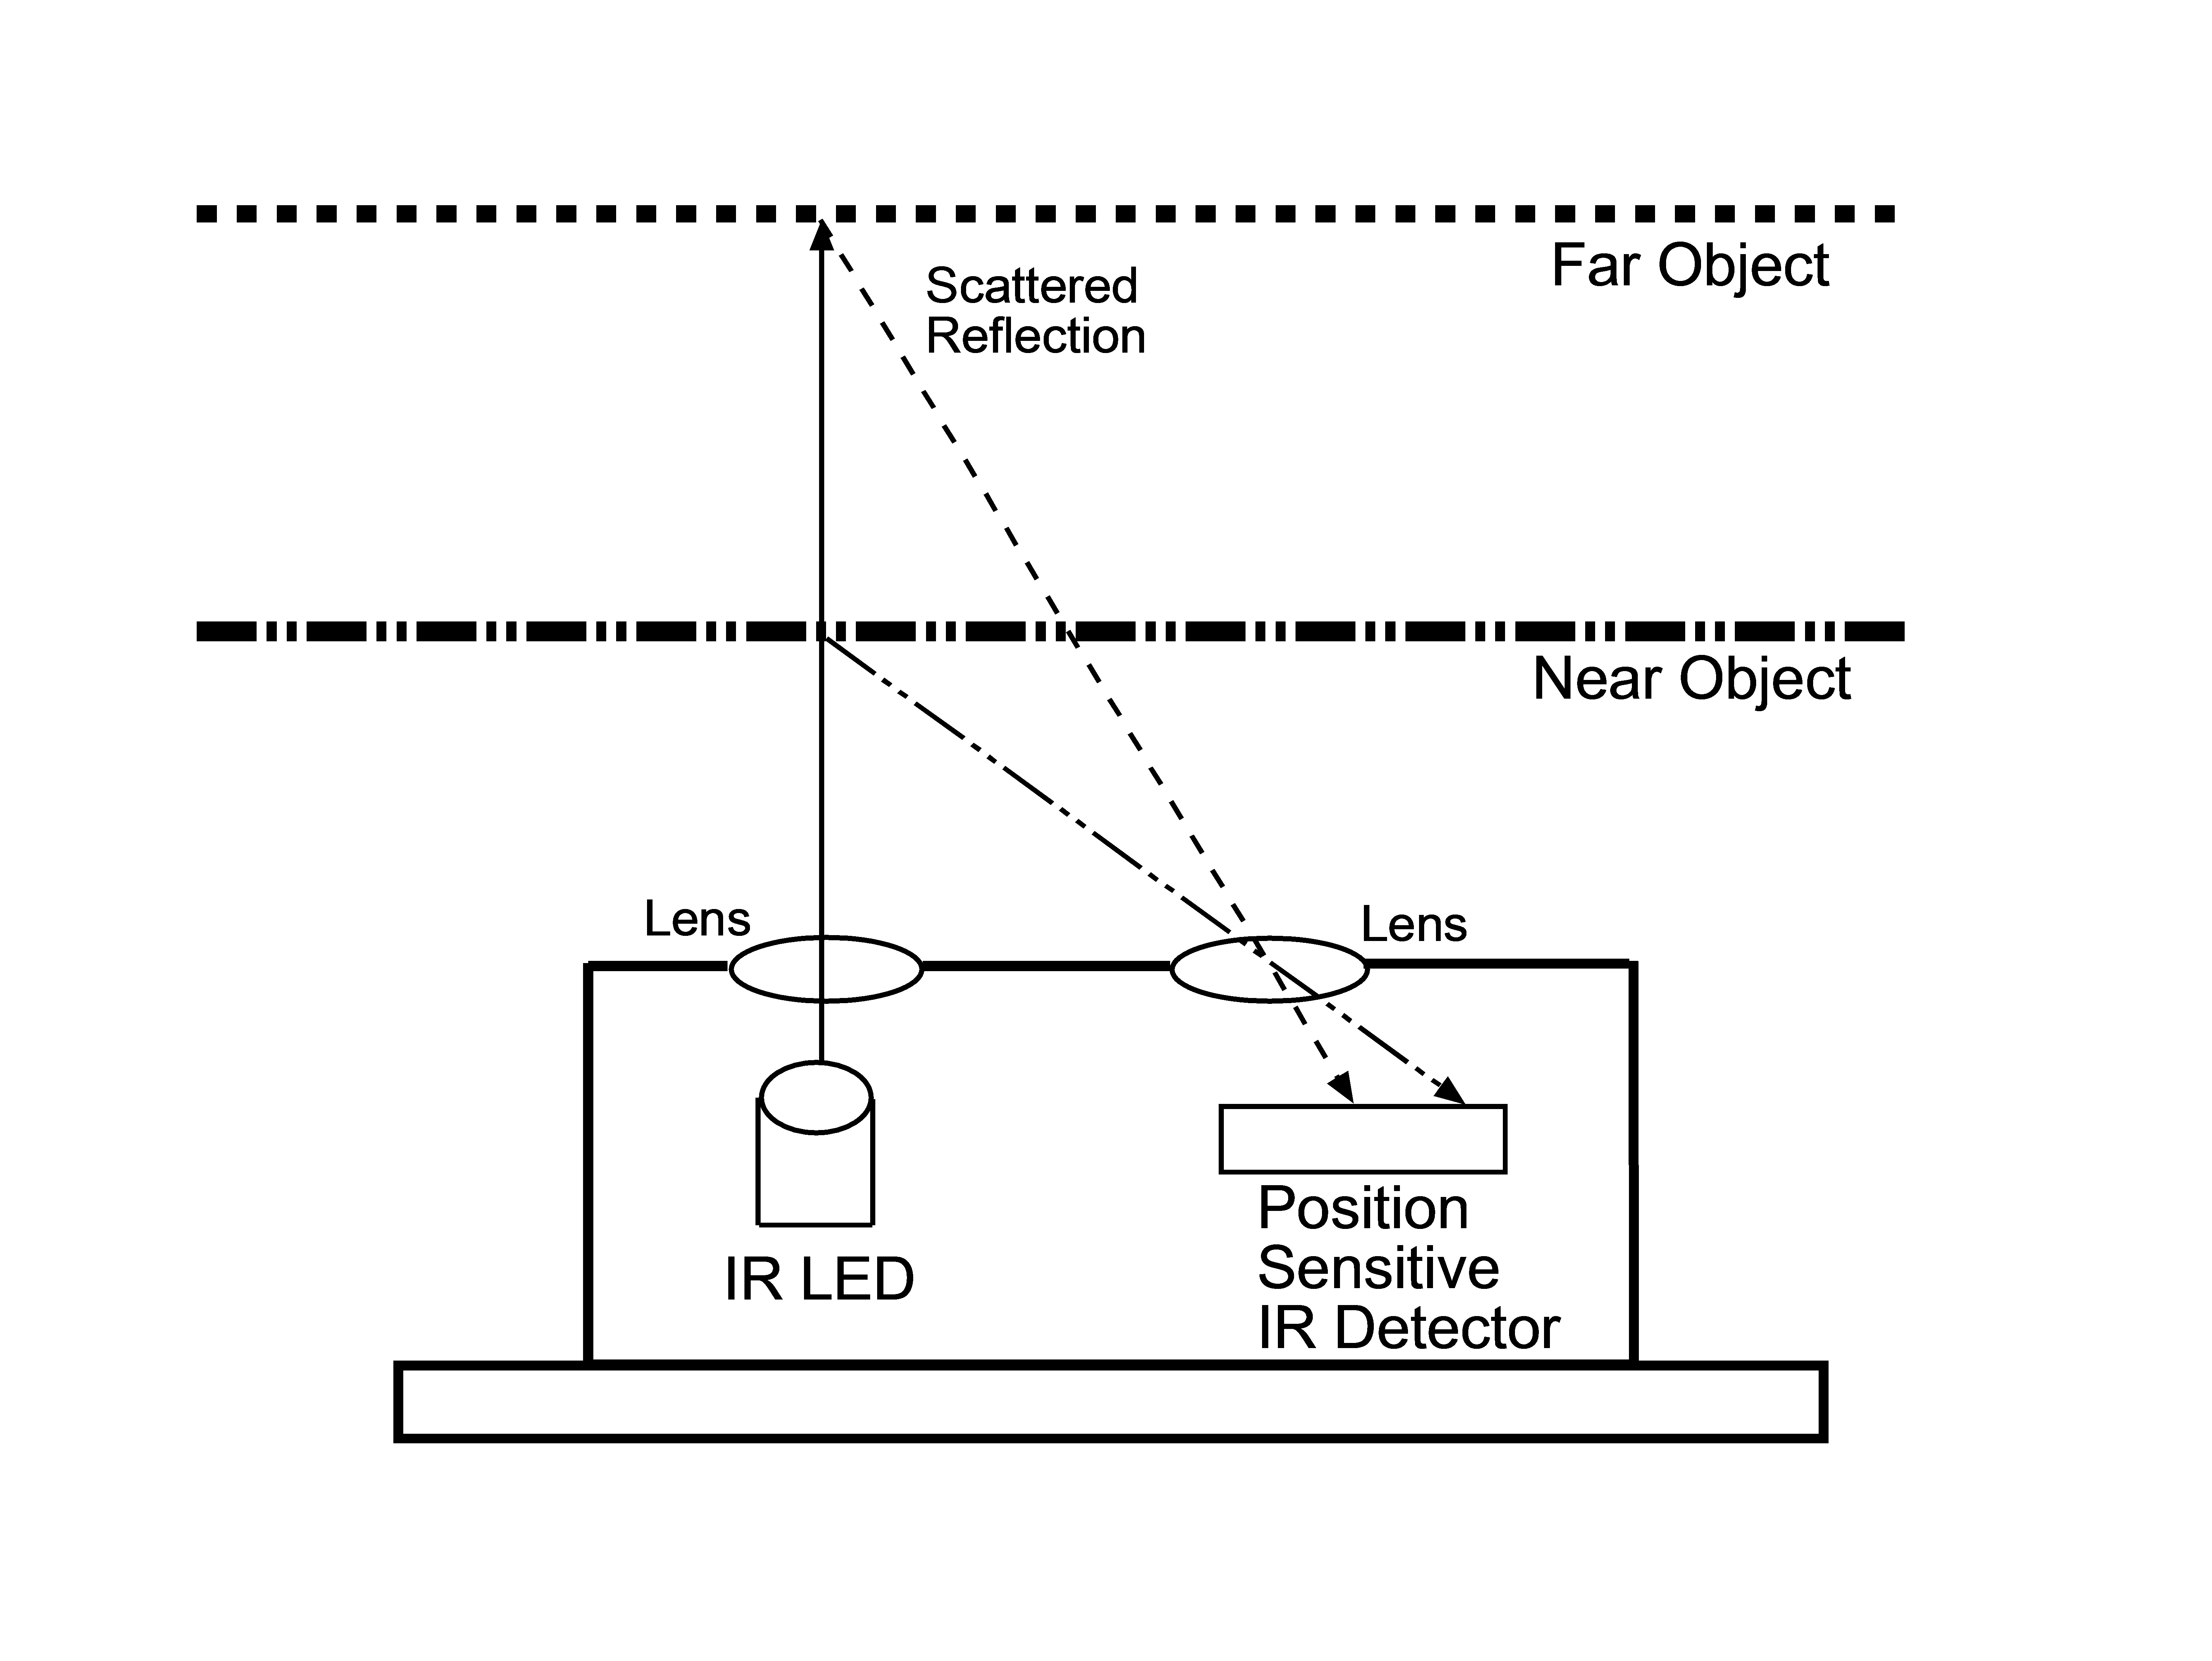
\includegraphics[width=.4\linewidth]{images/rangefinder.jpg}
        \caption{A slightly more complex laser rangefinder.}
        \label{fig:rangefinderIMG}
\end{figure}

This requires the rangefinder to know what the speed of the pulse is, which is a problem in unknown environments. For a rangefinder to be reliably used in such environments, it needs either to have the speed of its pulse precalculated, or it needs to measure the speed of the pulse by itself. Also, in situations where the speed of the pulse varies, a rangefinder is either not useful, or it needs a more complicated model of the environment it is in.

The main cause for a pulse to travel at a different speed than expected is in situations where the environment the sensor is in varies in density, which depends on temperature\cite{refraction}. Hence, a simple rangefinder is not fit for an environment that varies heavily in temperature.

Sound moves faster through denser mediums, where light travels slower. The speed of light is less affected by density than sound is. In earth-like atmospheres, light only travels 0.03\% slower in air when compared to the vacuum.\cite{refraction}\cite{speedOfSound}.

Another issue in environments with a high variation in density is refraction. Refraction is a phenomenon that occurs when a wave switches between mediums where it travels at different speeds. This change in mediums causes the wave to change it's direction. \cite{snell} Refraction would cause rangefinders to become effectively blind, as neither their direction nor the length measured can be trusted.
%A cite needs to be fixed above - Thomas
\begin{figure}[H]
	\centering
	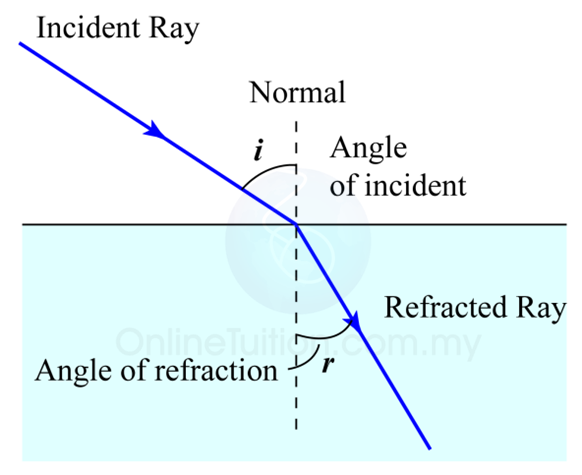
\includegraphics[width=.4\linewidth]{images/refraction.png}
        \caption{An illustration of refraction into a denser medium.}
        \label{fig:refractionIMG}
\end{figure}

